\chapter{THỰC NGHIỆM VÀ ĐÁNH GIÁ} %Implementation and Evaluation

\section{Thực nghiệm}

    Ta sẽ tiến hành thực nghiệm trình thông dịch cho ngôn ngữ Pandora bằng cách viết một số chương trình bằng chính ngôn ngữ Pandora, sau đó sử dụng trình thông dịch để xử lý tệp và kiểm chứng kết quả. Sau đây là một số kết quả khi chạy các chương trình khác nhau:

\subsection{Chương trình "Hello, World"}

\begin{figure}[H]
    \centering
    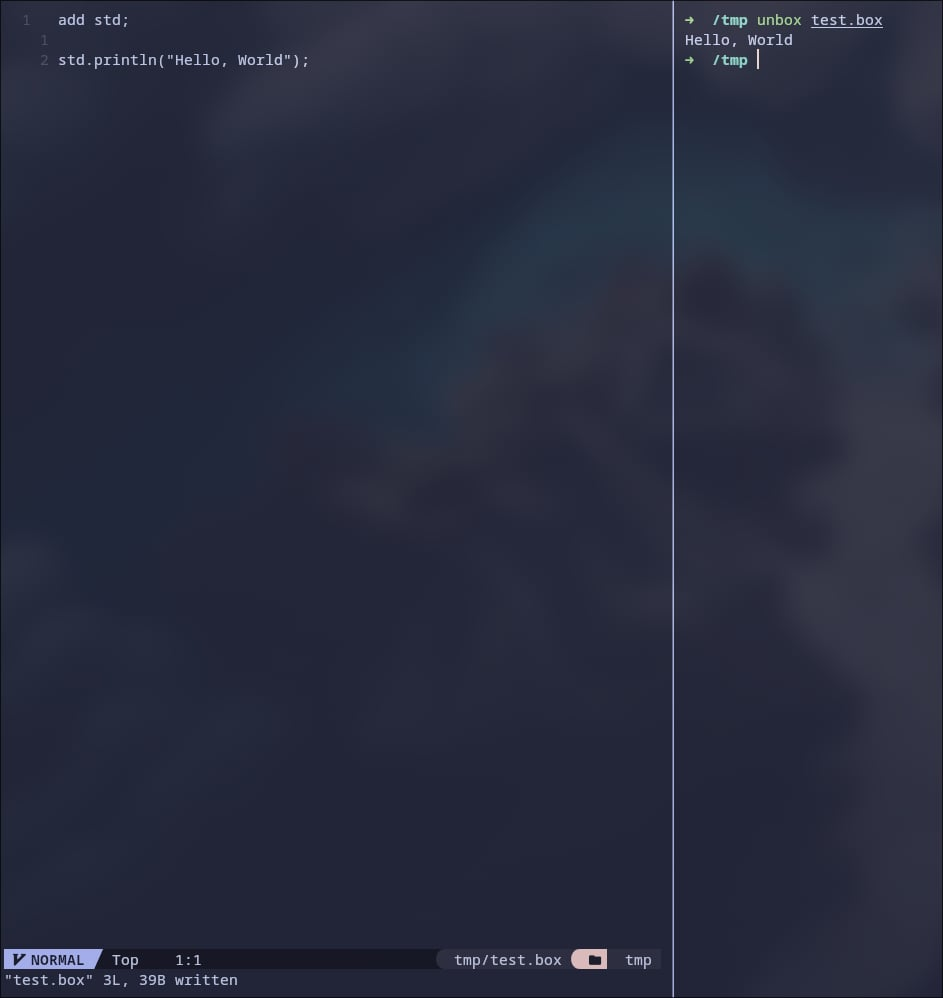
\includegraphics[scale=0.46]{test-prod-1.jpg}
    \caption{Ví dụ chạy chương trình in ra "Hello, World"}
\end{figure}

    Kết quả: chương trình sau khi thực thi đã in ra màn hình một cách chính xác kết quả là "Hello, World".

\subsection{Chương trình tính số fibonacci}

\begin{figure}[H]
    \centering
    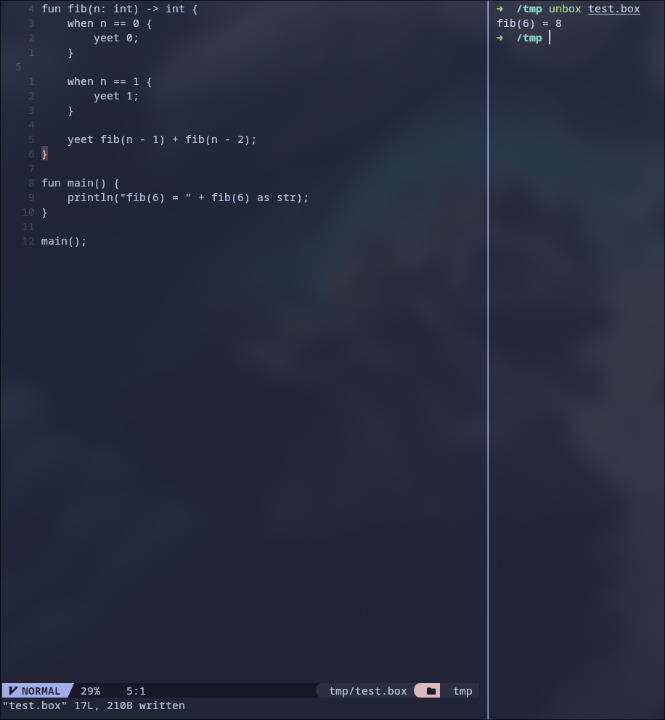
\includegraphics[scale=0.64]{test-prod-2.jpg}
    \caption{Ví dụ chạy chương trình tính fibonacci}
\end{figure}

    Kết quả: chương trình sau khi thực thi đã tính đúng số fibonacci và in ra màn hình như mong đợi.

\subsection{Chương trình sắp xếp nổi bọt}

\begin{figure}[H]
    \centering
    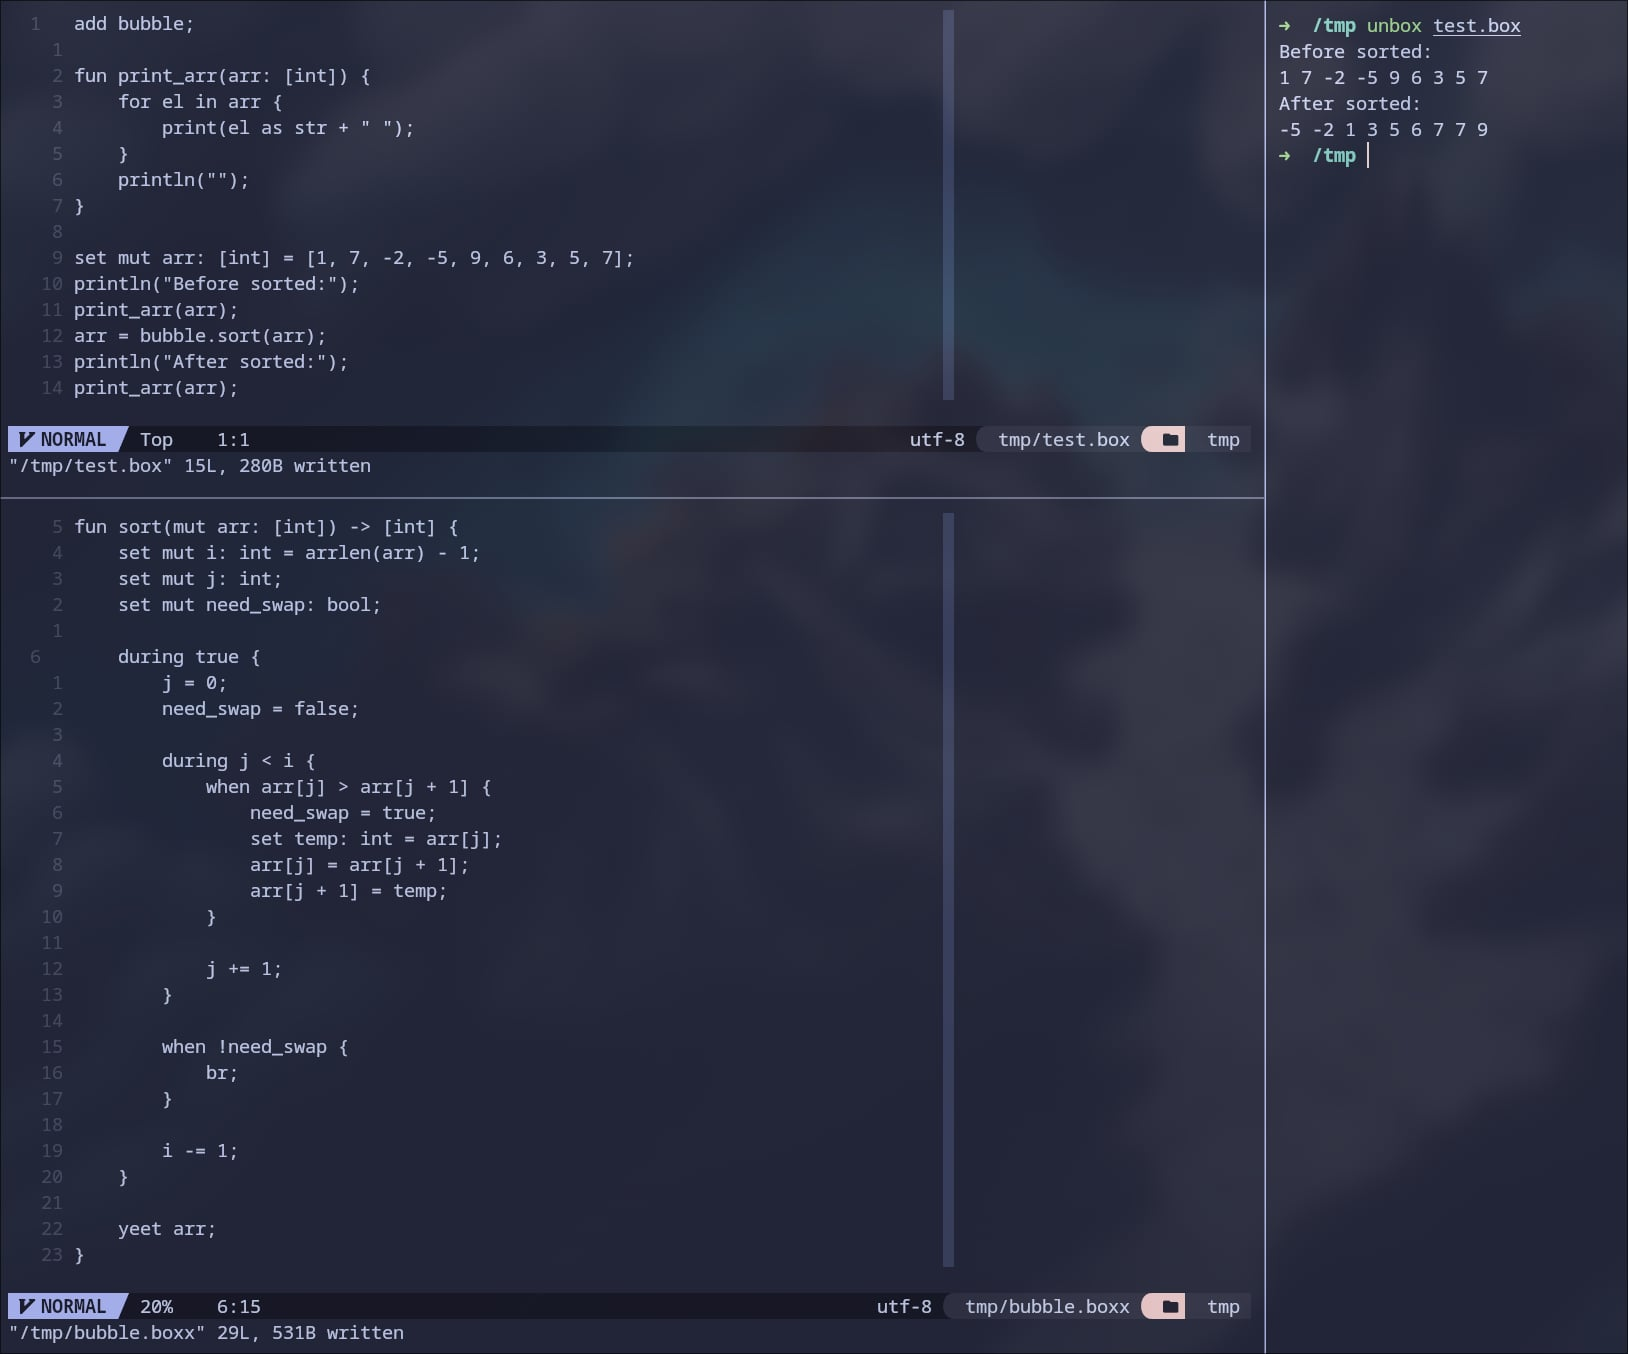
\includegraphics[scale=0.255]{test-prod-3.jpg}
    \caption{Ví dụ chạy chương trình sắp xếp nổi bọt}
\end{figure}

    Kết quả: chương trình sau khi thực thi đã in ra mảng được sắp xếp một cách chính xác.

\subsection{Chương trình sai từ vựng}

\begin{figure}[H]
    \centering
    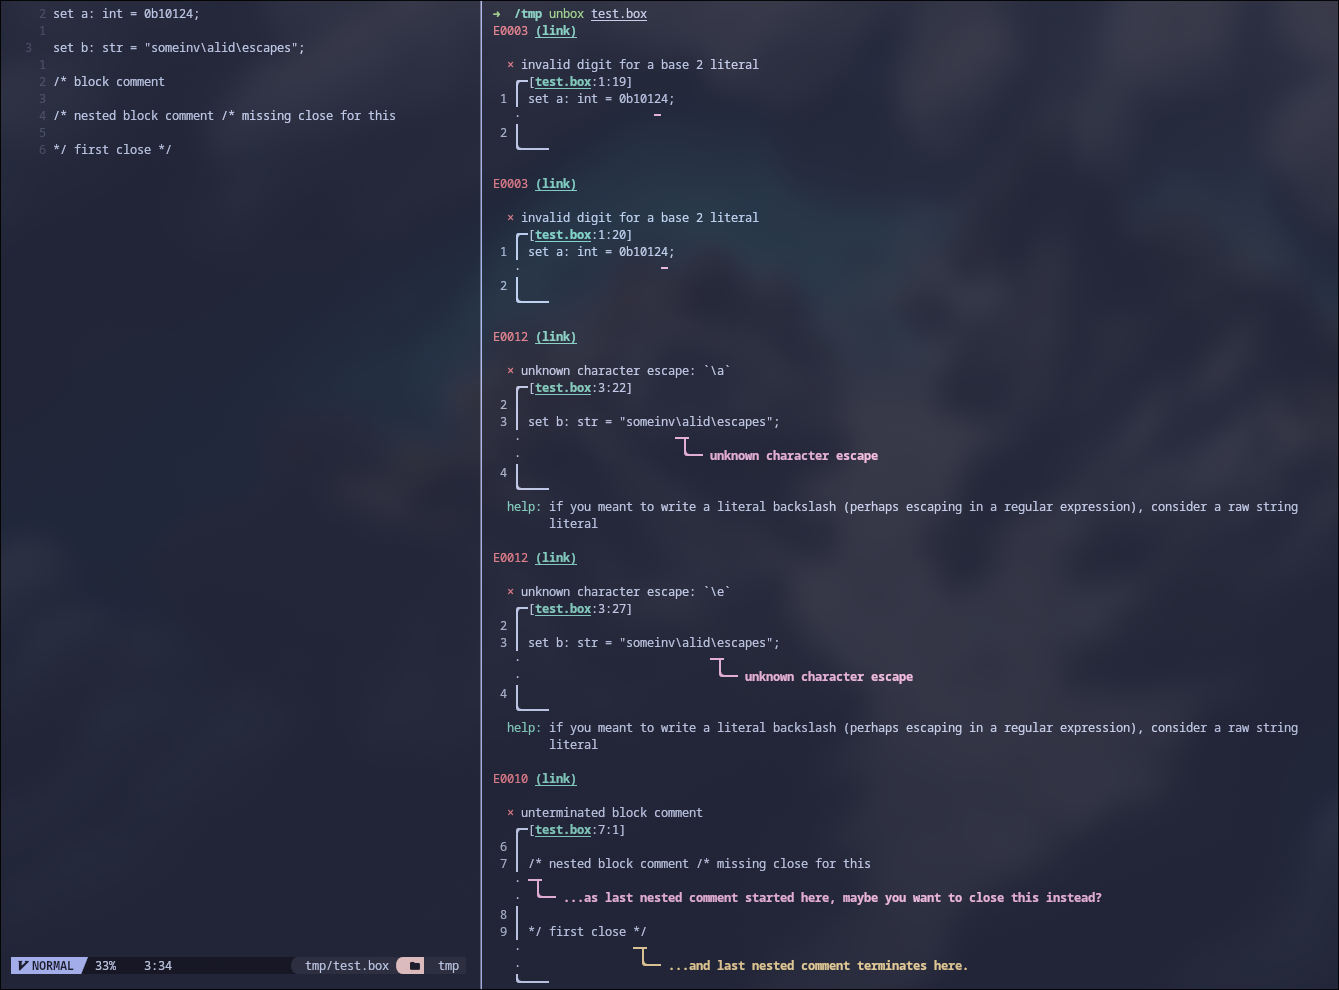
\includegraphics[scale=0.315]{test-prod-4.png}
    \caption{Ví dụ chạy chương trình sai từ vựng}
\end{figure}

    Kết quả: chương trình sau khi thực thi sẽ thông báo các lỗi từ vựng như ta mong muốn.

\subsection{Chương trình sai cú pháp}

\begin{figure}[H]
    \centering
    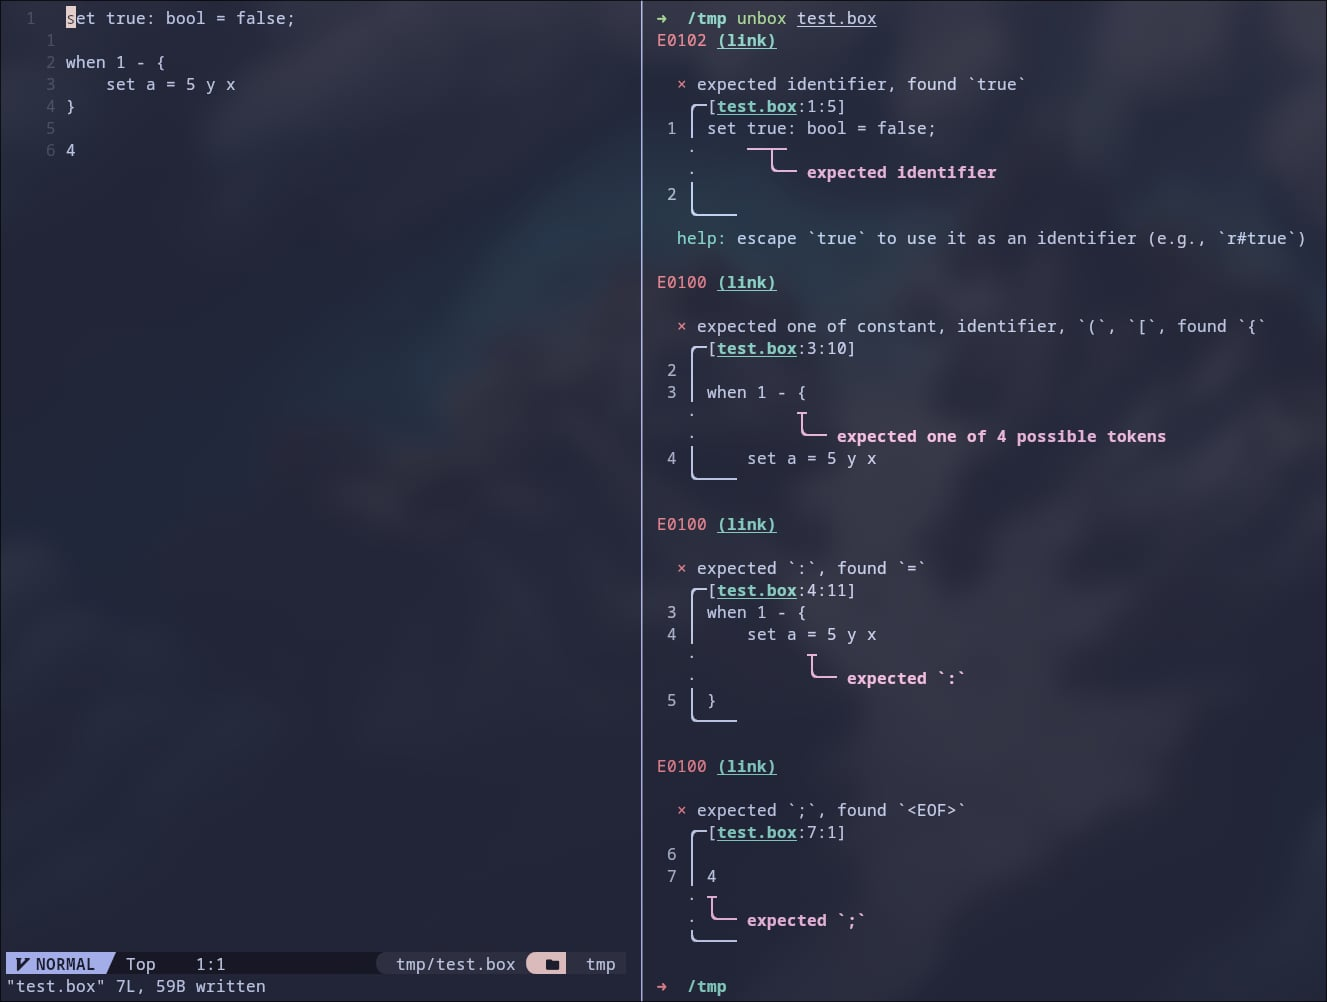
\includegraphics[scale=0.315]{test-prod-5.jpg}
    \caption{Ví dụ chạy chương trình sai cú pháp}
\end{figure}

    Kết quả: chương trình sau khi thực thi sẽ thông báo các lỗi cú pháp như ta mong muốn.

\subsection{Chương trình sai ngữ nghĩa}

\begin{figure}[H]
    \centering
    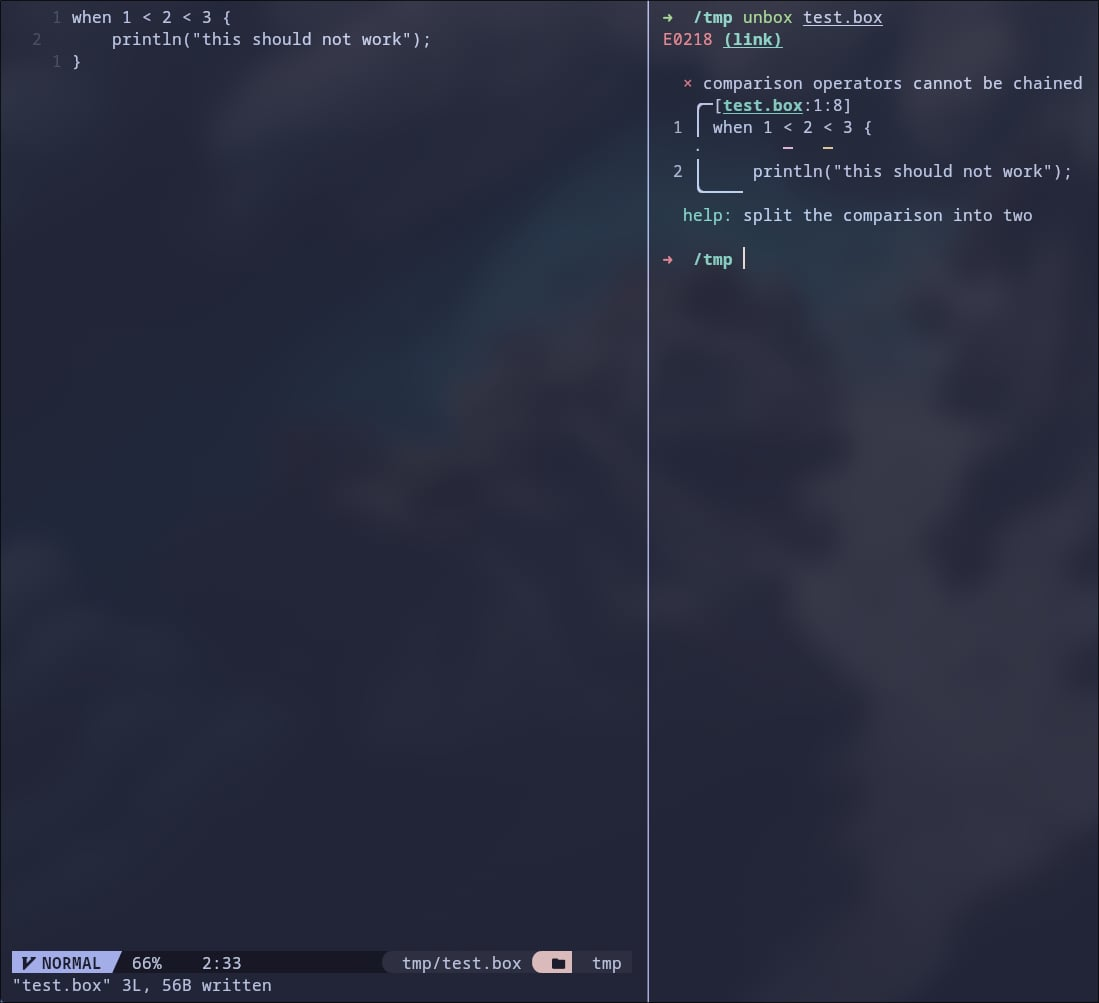
\includegraphics[scale=0.38]{test-prod-6.jpg}
    \caption{Ví dụ chạy chương trình sai ngữ nghĩa}
\end{figure}

    Kết quả: chương trình sau khi thực thi sẽ thông báo các lỗi ngữ nghĩa như ta mong muốn.

\subsection{Chương trình sắp xếp nổi bọt ở chế độ hỗn loạn}

\begin{figure}[H]
    \centering
    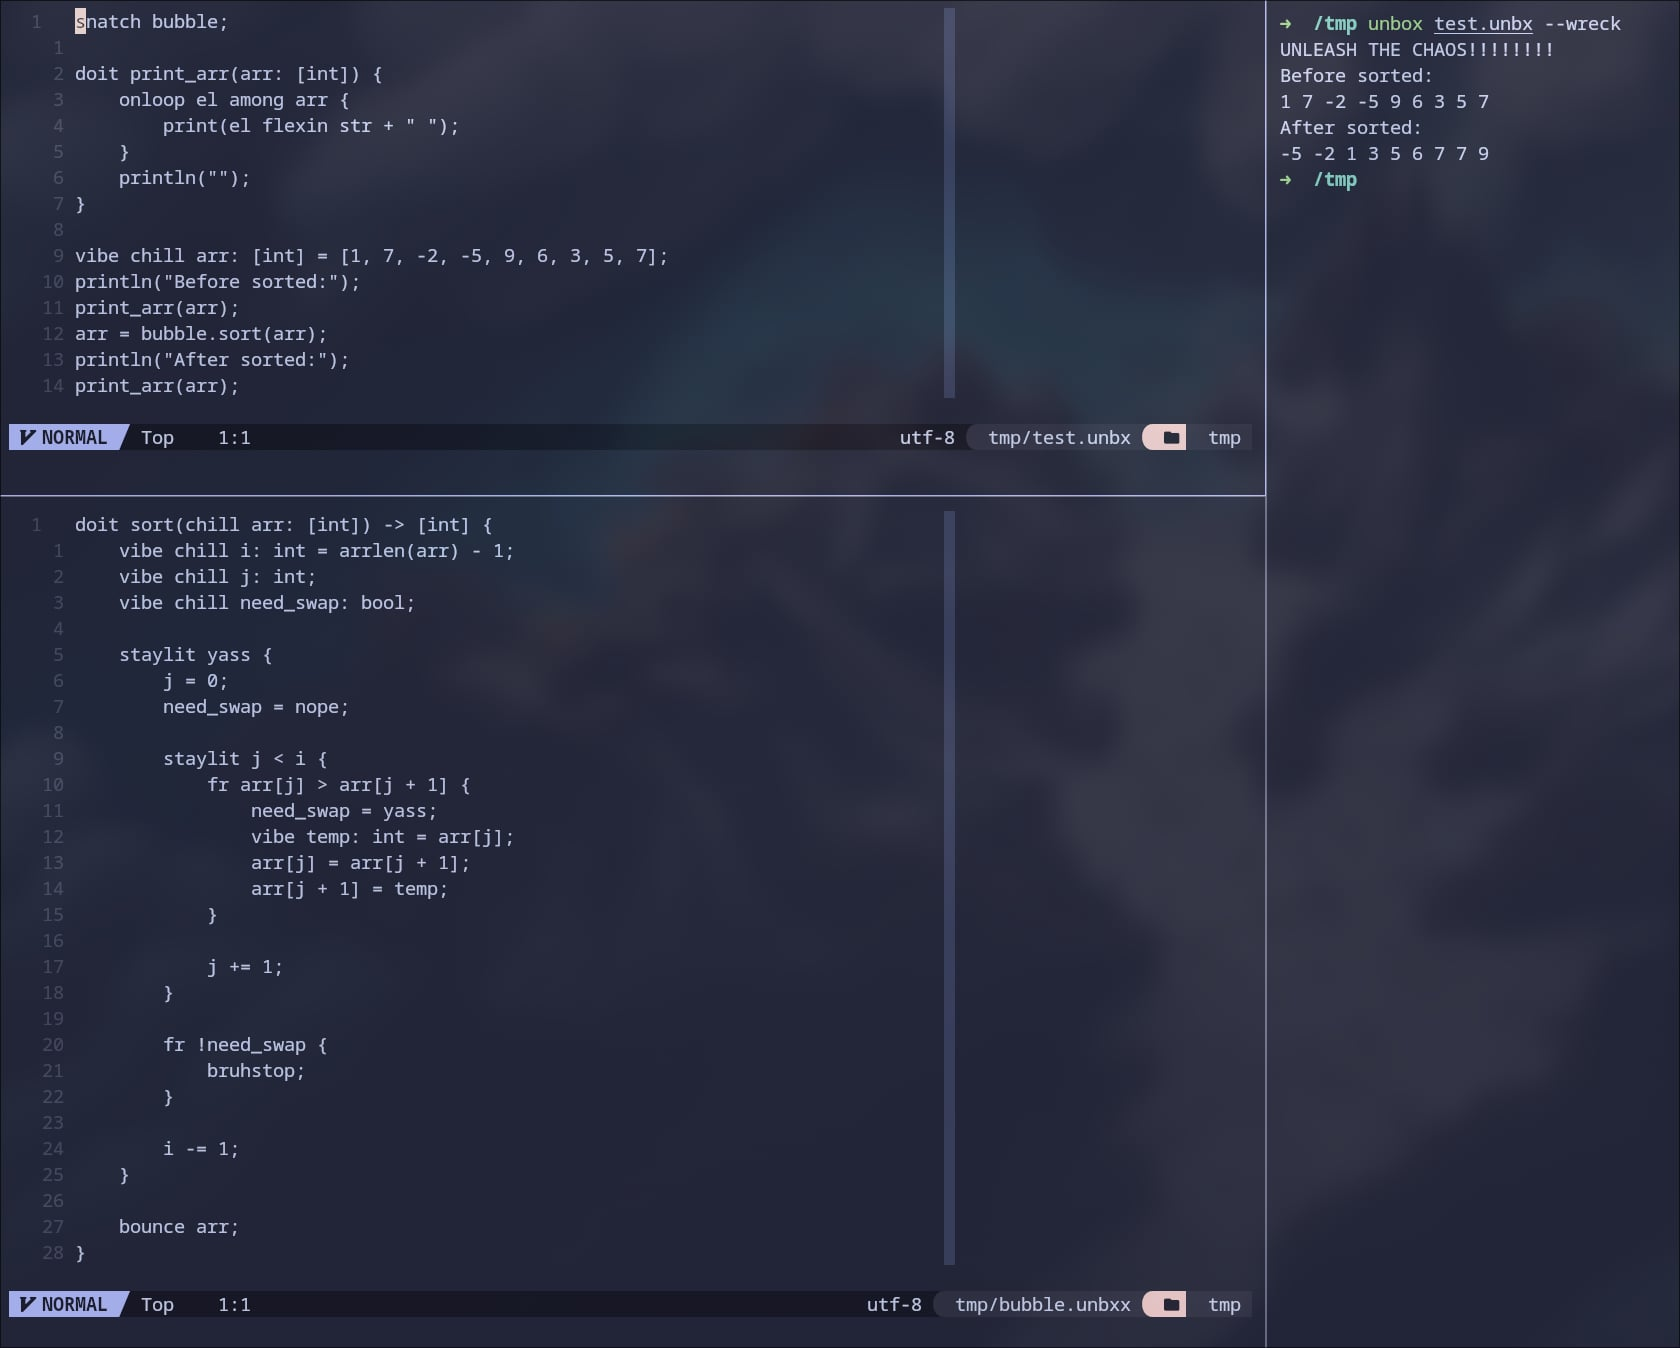
\includegraphics[scale=0.245]{test-prod-7.jpg}
    \caption{Ví dụ chạy chương trình sắp xếp nổi bọt ở chế độ hỗn loạn}
\end{figure}

    Kết quả: chương trình sau khi thực thi sẽ in ra mảng được sắp xếp một cách chính xác.

\section{Đánh giá}

    Từ kết quả thực nghiệm trên, ta có thể thấy rằng trình thông dịch Pandora đã hoạt động một cách chính xác và hiệu quả. Trình thông dịch đã xử lý các lỗi từ vựng, cú pháp và ngữ nghĩa đúng như chúng ta đã mong đợi. Điều này chứng tỏ rằng trình thông dịch Pandora đã hoạt động tốt và đáp ứng được các mục tiêu, yêu cầu đã đề ra. Các thực nghiệm trên cũng đã chứng tỏ tính đúng đắn, hiệu quả và linh hoạt của ngôn ngữ Pandora, giúp người dùng dễ dàng sử dụng và hiểu được ngôn ngữ này.
